%%%%%%%%%%%%%%%%%%%%%%%%%%%%%%%%%%%%%%%%%%%%%%%
%%%This is a science homework template. Modify the preamble to suit your needs. 
%The junk text is   there for you to immediately see how the headers/footers look at first 
%typesetting.


\documentclass{article}

%AMS-TeX packages
\usepackage{amssymb,amsmath,amsthm} 
%geometry (sets margin) and other useful packages
\usepackage[margin=1.25in]{geometry}
\usepackage{graphicx,ctable,booktabs}
\usepackage{enumerate}
\usepackage{bbm}
\usepackage{courier}
\usepackage{centernot}

%\usepackage{algorithmicx}
\usepackage{algorithm}
\usepackage{algpseudocode}

\algblockx[Name]{Start}{End}
{}
{}

% For pretty python code
\usepackage{fancyvrb}
\usepackage{color}
\usepackage[latin1]{inputenc}
\usepackage{minibox}

%Probability and Expectation
\newcommand{\Ex}[2]{\underset{#2}{\mbox{E}}\!\left[#1\right]}
\newcommand{\Exhat}[2]{\underset{#2}{\hat{\mbox{E}}}\!\left[#1\right]}
\renewcommand{\Pr}[1]{\mbox{P}\!\left(#1\right)}
\newcommand{\Prob}[2]{\underset{#2}{\mbox{Pr}}\!\left[#1\right]}
\newcommand{\Var}[2]{\underset{#2}{\mbox{Var}}\!\left(#1\right)}

\newcommand{\abs}[1]{\left|#1\right|}

%
%Fancy-header package to modify header/page numbering 
%
\usepackage{fancyhdr}
\pagestyle{fancy}
%\4addtolength{\headwidth}{\marginparsep} %these change header-rule width
%\addtolength{\headwidth}{\marginparwidth}
\chead{} 
\lhead{R. Hasegawa}
\rhead{\thepage} 
\lfoot{\small\scshape Advanced Monte Carlo Methods - Sp2013} 
\cfoot{} 
\rfoot{\footnotesize Final Project} 
\renewcommand{\headrulewidth}{.3pt} 
\renewcommand{\footrulewidth}{.3pt}
\setlength\voffset{-0.25in}
\setlength\textheight{648pt}

%%%%%%%%%%%%%%%%%%%%%%%%%%%%%%%%%%%%%%%%%%%%%%%

%
%Contents of problem set
%    
\begin{document}

\title{A Correctness Analysis of the Stochastic Gradient Langevin Descent Algorithm}
\author{Raiden Hasegawa}
\date{May 21, 2013}

\maketitle

\thispagestyle{empty}
%\setcounter{section}{}

\begin{section}{Introduction}
In this short paper I investigate whether the Stochastic Gradient Langevin Descent (SGLD) algorithm presented in \cite{WelTeh2011a} for Bayesian posterior sampling is exact or not.  A straightforward error analysis suggests that the method will be biased and the number of expected rejections will be on the order of $O(N/n)$ even when the step size is annealed to zero, where $N$ is the size of the dataset and $n$ is the size of the batch.  Several experiments with the same toy model presented in the original paper corroborate this and show that the Monte Carlo estimates produced by SGLD are very sensitive to the batch size and the choice of the annealing schedule.  The experiments do suggest that SGLD estimates may improve as as the ratio $N/n$ decreases.
\end{section}
\begin{section}{Algorithm and Analysis}
\begin{subsection}{\it Langevin Monte Carlo (LMC)}
Consider a Bayesian model with parameters $\theta$, data $X=\{X_i\}_{i=1}^N$ and a posterior that can be expressed as 
\begin{equation}
\mathcal{P}(\theta | X) = \Pr{\theta}{}\prod_{i=1}^N \Pr{X_i | \theta}{} \,. \label{post}
\end{equation}
This implies that the likelihood function $\mathcal{L}(X | \theta)$ is separable over the data which is a reasonable assumption.  The Monte Carlo proposal using Langevin dynamics can be expressed as
\begin{equation}
\theta_{t+1} = \theta_t + \frac{\epsilon}{2}\left\{\nabla \log\{\Pr{\theta}\} +  \sum_{i=1}^N \nabla \log\{ \Pr{X_i | \theta}\}\right\}+ \eta\,, \quad \eta \sim \mathcal{N}(0,\epsilon) \,. \label{LMC}
\end{equation}
Since we end up with a discretization error of $\epsilon^{3/2}$ (which I prove below), a Metropolis Hastings (MH) rejection step needs to be introduced to ensure detailed balance.
\end{subsection}
\begin{subsection}{\it Stochastic Gradient Langevin Descent (SGLD)}
In a sampling setting where our likelihood involves the evaluation over a massive number of data points, \eqref{LMC} becomes infeasible.  At every step we need to evaluate the full likelihood (or gradient thereof) to make the step and then again to decide whether or not to reject.  Given Monte Carlo solutions converge at a rate of $O(1/\sqrt{T})$ \cite{Liu01}, \eqref{LMC} is only useful for relatively small problems.  \cite{WelTeh2011a} proposes a potential remedy to this ``curse of big data" problem by approximating \eqref{LMC} using ideas from Stochastic Gradient Descent (SGD).  They make a few claims that the noise from approximating the gradient in \eqref{LMC} with a random batch of the full data is eventually dominated by the injected noise term $\eta$ when $\epsilon$ follows a polynomial annealing schedule. Thus , SGLD should eventually sample from the correct distribution.  Critical to their claim is that the discretization error will go to zero as $\epsilon$ is annealed to zero, thus eliminating the need for a costly MH step.  The algorithm can be summarized by the following proposal step
\begin{equation}
\theta_{t+1} = \theta_t + \frac{\epsilon_t}{2}\left\{\nabla \log\{\Pr{\theta}\} +  \frac{N}{n}\sum_{i=1}^n \nabla \log\{ \Pr{X_i | \theta}\}\right\}+ \eta\,, \quad \eta_t \sim \mathcal{N}(0,\epsilon_t) \,. \label{SGLD}
\end{equation}
A batch size of $n$ random data is used to approximate the likelihood gradient.  The step size, $\epsilon_t$ follows a polynomial annealing schedule such that the SGLD should end up near a mode.
\begin{subsubsection}{\it Concerns}
At first look, this approximation looks promising given the success of SGD in maximization problems \cite{Bottou10}.  The gist of their claim is that SGLD takes the best of both worlds: efficient maximization using SGD while generating a sample from the Bayesian posterior.  But, a closer analysis reveals some potential problems.  First, the fact that the algorithm avoids the costly MH step because the discretization error of the SGLD step goes to zero as $\epsilon$ is annealed is not a free lunch.  The cost for avoiding the MH step is extremely long autocorrelation times since we end up with very small steps.  I observe this in the results of my experiments.  Secondly, the probability of rejection may go to zero with $\epsilon$ but it is not the case that the expected number of rejections over a sampling run will asymptotically approach zero as well.  In fact, I show below that one should expect a non-trivial number of rejections over a sampling run, introducing bias into our Monte Carlo estimates.
\end{subsubsection}
\end{subsection}

\begin{subsection}{\it Error Analysis}
I will first show that as $\epsilon \to 0$ the expected number of rejections goes to zero when the full Posterior is evaluated at each Langevin proposal.  Then, we will show why this does not hold for SGLD and that one should expect this method to be biased.  Consider the Hamiltonian where the negative log-posterior is the potential energy function:
\begin{equation} 
H(\theta,\rho) = -\log\{\mathcal{P}(\theta|X)\} + \frac{1}{2}\rho^2 \,. \label{ham}
\end{equation}
The join probability function can be expressed as $\frac{1}{Z}\exp\{ -H(\theta,\rho) \}$. Recall that the time dynamics of $\theta$ and $\rho$ can be related to the hamiltonian defined in \eqref{ham} by the following Hamiltonian equations:
\begin{equation}
\frac{d \theta}{dt}  = \rho\quad, \quad \frac{d \rho}{dt}  = \frac{\partial \log\{\mathcal{P}\}}{\partial \theta} \label{dHam}
\end{equation}
For simplicity, we will work with the case where $\theta$ and $\rho$ are of dimension 1.  The uncorrected Langevin proposal has the following steps
\begin{enumerate}
\item draw $\rho$ from $\mathcal{N}(0,1)$.
\item Make the following Langevin update (equivalent to a single Leapfrog update for a Hamiltonian Monte Carlo scheme \cite{Neal10}:
\begin{align}
\theta^*&  = \theta + \frac{\epsilon}{2} \frac{\partial  \log\{\mathcal{P}\}}{\partial \theta}(\theta) + \sqrt{\epsilon} \rho \label{dLt}\\
\rho^*&  = \rho+ \frac{\sqrt{\epsilon}}{2} \frac{\partial  \log\{\mathcal{P}\}}{\partial \theta}(\theta) + \frac{\sqrt{\epsilon}}{2} \frac{\partial \log\{\mathcal{P}\}}{\partial \theta}(\theta^*)  \label{dLp} \\
\end{align}
\end{enumerate}
When we add a MH step to correct for the discretization error in moving along the Hamiltonian in step (2), both steps preserves the invariant distribution.  Step (2) can be rewritten as the three steps of the symplectic Leapfrog integrator which is reversible and preserves volume \cite{Neal10}.Now see that the taylor expansion of $\theta(t+\sqrt{\epsilon})$ and $\rho(t+\sqrt{\epsilon})$ at $t$ can be written as
\begin{align}
\theta(t+\sqrt{\epsilon}) & = \theta(t) + \sqrt{\epsilon} \frac{d \theta}{dt}(t) + \frac{\epsilon}{2}\frac{d^2\theta}{dt^2}(t) + O(\epsilon^{3/2}) \label{tay_t} \\
\rho(t+\sqrt{\epsilon}) & = \rho(t) + \sqrt{\epsilon} \frac{d \rho}{dt}(t) + \frac{\epsilon}{2}\frac{d^2\rho}{dt^2}(t) + O(\epsilon^{3/2}) \label{tay_p}
\end{align}
Using the Hamiltonian differential equations in \eqref{dHam} and noting that $$\frac{d}{dt}\frac{d \theta}{dt}  = \frac{d \rho}{dt} =  \frac{\partial \log\{\mathcal{P}\}}{\partial \theta}$$ we see that the discretization error for $\theta$ is  
\begin{equation}
\theta^* - \theta(t+\sqrt{\epsilon}) = O(\epsilon^{3/2})\,. \label{err_t}
\end{equation}
The analysis for $\rho$ is a little trickier but the end result is the same in terms of the error.  Consider the taylor expansion of $\frac{\partial \log\{\mathcal{P}\}}{\partial \theta}$
\begin{align}
\frac{\partial \log\{\mathcal{P}\}}{\partial \theta}(t+\sqrt{\epsilon}) & = \frac{\partial \log\{\mathcal{P}\}}{\partial \theta}(t) + \sqrt{\epsilon}\frac{\partial}{\partial t}\frac{\partial \log\{\mathcal{P}\}}{\partial \theta}(t) + O(\epsilon) \notag \\
\implies \frac{\partial \log\{\mathcal{P}\}}{\partial \theta}(\theta^*) & = \frac{\partial \log\{\mathcal{P}\}}{\partial \theta}(\theta) + \sqrt{\epsilon}\frac{\partial}{\partial t}\frac{\partial \log\{\mathcal{P}\}}{\partial \theta}(\theta) + O(\epsilon) \label{rho2}
\end{align}
The second line holds since the first of our Langevin equations for $\theta$ defines the following map $(t,t+\sqrt{\epsilon}) \mapsto (\theta,\theta^*)$.  Inserting \eqref{rho2} into \eqref{dLp} gives us
\begin{align}
\rho^*  & = \rho+ \sqrt{\epsilon}\frac{\partial  \log\{\mathcal{P}\}}{\partial \theta}(\theta) + \frac{\epsilon}{2} \frac{\partial}{\partial t} \frac{\partial \log\{\mathcal{P}\}}{\partial \theta}(\theta) + O(\epsilon^{3/2}) \notag \\
& = \rho+ \sqrt{\epsilon}\frac{\partial \rho}{\partial t}(t) + \frac{\epsilon}{2} \frac{\partial^2\rho}{\partial t^2}(t) + O(\epsilon^{3/2}) \,. \label{dLp2}
\end{align}
Thus, we see that the discretization error for $\rho$ is also of the form
\begin{equation}
\rho^* - \rho(t+\sqrt{\epsilon}) = O(\epsilon^{3/2})\,. \label{err_p}
\end{equation}
When $H(\theta,\rho)$ is well behaved with respect to $\theta$ and $\rho$ (e.g. Lipschitz) then our discretization error for $H(\theta,\rho)$ should also be $O(\epsilon^{3/2})$ leading to rejection probabilities of the same order of magnitude.  Since LMC exhibits random walk behavior, the number of steps to traverse some given distance will be $O(1/\epsilon)$ \cite{Neal93}.  Thus, the expected number of rejections should be $O(\sqrt{\epsilon})$ which goes to zero as $\epsilon$ goes to zero.
\begin{subsubsection}{\it Bias in SGLD}
The above analysis suggests we should get an unbiased estimate using LMC without an MH step when our $\epsilon$ is small.  Although not important to the current point I am trying to make, this observation isn't terribly useful since the growth in autocorrelation time may offset any computational gains from avoiding a rejection step.  Back to the point I am trying to make, SGLD as defined in \eqref{SGLD} will have discretization error dominated by the approximated gradient, which will be of order $O(\epsilon (N/n))$.  This is troublesome in that, the expected number of rejections as $\epsilon \to 0$ is no longer zero. It will be nontrivial and of order $O(N/n)$.  This suggests that even if we anneal our step size to zero, SGLD will be asymptotically biased.  In the following section I run some experiments that seems to validate this claim.
\end{subsubsection}
\end{subsection}
\end{section}
\begin{section}{Experiment}
In this section I will briefly describe the tests of correctness for SGLD.  In summary, I compute the ``true" probability of three different regions of a toy posterior and compare the probability derived from the SGLD sampler with varying parameters.  As a baseline, I also generate draws using a corrected LMC sampler which in theory should be exact.
\begin{subsection}{\it Toy Model}
The toy model used in \cite{WelTeh2011a} is a posterior defined by Gaussian priors and a likelihood that is a mixture of two Gaussians.  The model is parameterized in such a way that the two parameters we are sampling are very negatively correlated and the bivariate posterior tends to be bimodal, depending of course, on the data.  The model is as follows
\begin{align}
& \theta_1 \sim \mathcal{N}(0,\sigma_1^2)\,; \quad \theta_2 \sim \mathcal{N}(0,\sigma_2^2) \notag \\
& x_i \sim \frac{1}{2}\mathcal{N}(\theta_1,\sigma_x^2) + \frac{1}{2}\mathcal{N}(\theta_1+\theta_2,\sigma_x^2) \notag
\end{align}
where $\sigma_1^2=10$, $\sigma_2^2=1$, and $\sigma_x^2=2$.  The data are generated from the likelihood model where $\theta_1=0$ and $\theta_2=1$.  As mentioned in (\cite{WelTeh2011a}.  This construction should lead to a bimodal distribution as the number of data $N$ increases, with modes at $(\theta_1,\theta_2) = (0,1)$ and $(\theta_1,\theta_2) = (1,-1)$ since the likelihood function is invariant under these two cases.
\end{subsection}
\begin{subsection}{\it Test Statistic}
Three regions, $\{R_i:\,i\in[1,3]\}$, of the posterior distribution for $\theta_1$ and $\theta_2$ are chosen to construct our test statistics used to evaluate the exactness of the SGLD algorithm.  Using a trapezoidal integration scheme with a $1000\times1000$ grid I compute $\Prob{R_i}{}$ for each $i$.  Since the normalizing constant $Z$ is analytically intractable, we approximate it by using the same integration scheme over a large area that should contain nearly all the probability mass.  Since the trapezoidal rule has global error of order 2, our grid over $[-10,10]\times[-10,10]$ should result in an error with order of magnitude $10^{-4}$ which should be plenty of precision for our tests.  We should expect errors on the order of $10^{-3}$ from our correct sampling schemes when generating $10^6$ draws, and even larger when considering the autocorrelation time of the sequence of draws.  The results suggest errors that are closer to $10^{-2}$ for the correct sampler.  Our sampling estimates can be written as
\begin{equation}
\widehat{\Prob{R_i}{}}=\frac{\sum_{k=1}^n \mathbbm{1}_{R_i}(X_k)}{\sum_{k=1}^n \mathbbm{1}_{[-10,10]^2}(X_k)} \label{estPr}
\end{equation}
where the denominator corrects for the fact that our true value for $\Prob{R_i}{}$ is in fact a conditional probability.  Since our $\sum_{k=1}^n \mathbbm{1}_{R_i}$ follows a binomial distribution one can write the standard errors of $\widehat{\Prob{R_i}{}}$ as
\begin{equation}
\widehat{S.E.(\Prob{R_i}{})} = \left( \frac{\widehat{\Prob{R_i}{}}(1-\widehat{\Prob{R_i}{}})}{\left(\sum_{k=1}^n \mathbbm{1}_{[-10,10]^2}(X_k)\right)/\tau}\right)^{1/2} \label{se}
\end{equation}
where $\tau$ is the autocorrelation time of the function $\mathbbm{1}_{R_i}(X)$.
\end{subsection}
\begin{subsection}{\it Data}
For this experiment I use two artificially generated datasets (random seed = 17 and random seed = 19) according to the toy model both with $n=100$.  The first dataset, $D_1$, results in a unimodal posterior while the second, $D_2$ results in a bimodal posterior.  The unimodal posterior is centered on the prior but the peak is elongated by the likelihood between the two modes we expect.  By construction, both exhibit strong negative correlation between the $\theta$'s.  The posteriors are plotted below with regions $R_i$ indicated by the rectangles.  The three test regions are chosen along the length of the distribution such that the mode(s) should be accounted for and, in the case of multiple modes, separated by the regions.  You can see the posteriors for each distribution with the three regions identified in  {figure \ref{distr}}.
\begin{figure}[h!]
\caption{Posterior Distributions}
\label{distr}
\begin{center}
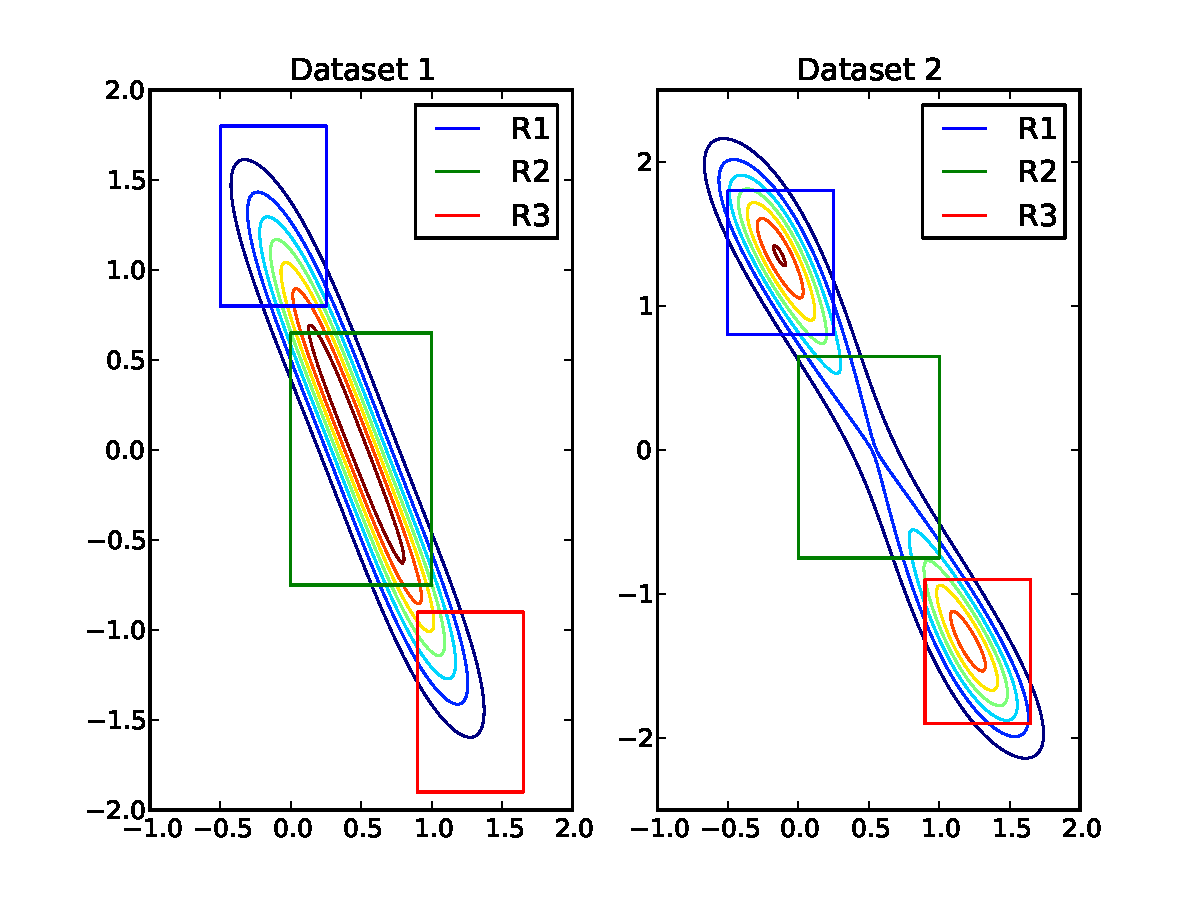
\includegraphics[scale=0.7]{../figures/distr_dataset.pdf}
\end{center}
\end{figure}
\end{subsection}

\begin{subsection}{\it Algorithm Specifications}
All algorithms generate $10^6$ draws.  As a baseline algorithm I use an LMC proposal move with an MH step to ensure detailed balance is satisfied.  I run the LMC sampler with several settings for $\epsilon$ (as defined in \eqref{LMC}).  The SGLD sampler is run with several batch sizes, $n$, and for several annealing schedules for $\epsilon$.  I use the polynomial schedule defined in \cite{WelTeh2011a}: $a(b+t)^{-\gamma}$ but change the maximum and minimum $\epsilon$.  This polynomial schedule meets the two following criteria that are required for SGD convergence to a mode \cite{Bottou10}:

$$ \sum_{t=1}^{\infty} \epsilon_t > \infty\,,\quad \sum_{t=1}^{\infty}\epsilon_t^2 < \infty\,.$$

Sampling from the data for each batch is done without replacement \cite{Niu11}.  For SGLD, I test the following batch sizes: $n = 1,2,4,8,16$.
\end{subsection}
\end{section}
\begin{section}{Results}
The results are summarized in figures \ref{lmc} to \ref{n16} that show the true statistic, estimated statistic and error bars for
$$\Prob{R_i}{D_j},\,i=1,2,3\text{ and }j=1,2$$
The first figure corresponds to the LMC sampler with the MH step while the next 6 correspond to the different batch sizes.  The estimated statistic is shown for different annealing schedules for SGLD and different fixed step sizes for LMC.  The figures for batch sizes $>1$ are in the appendix.

Considering our exact LMC sampler first in figure \ref{lmc} we see that for nearly every region and step size the true statistic falls within the error bars of our estimates.  This is what we wanted to see.  Given the narrow geometry and possibly low conductance of our posteriors (especiallin dataset $D_2$), these are the types of results one would expect and should be fairly satisfied with.  The key observation here is that the estimates seem to be reasonably stable with respect to the choice of $\epsilon$ and the estimator performs equally well for almost all the regions.  What's pleasant about these results is that it manages to sample well from both modes in $D_2$ even with bad geometry (see the first and third plot in the second column).

On the other hand, in figure \ref{n1} we see variable results from our SGLD with batch size of $1$ (Note that the scales are not the same between the LMC plots and the SGLD plots).  Few estimators catch the true statistic in their error bars and the estimates are very sensitive to annealing schedule.  Some schedules are too slow and end up with zero estimates. This may be the result of the sample chain bouncing back and forth over the narrow axis of the distribution.  As we might expect, the estimates seem to stabilize somewhat for $n=16$ (at least for the unimodal distribution).  But, this does not appear to be a monotonic effect with respect to $n$ and for larger $n$ we still see some bad annealing schedules.  The performance for all SGLD methods seems to be a bit better for the unimodal distribution $D_1$.

\cite{WelTeh2011a} also suggests a method to re-weight the estimates based on $\epsilon_t$ to account for the annealing schedule.  The intuition is that the effective sample size of a draw from the posterior is proportional to $\epsilon_t$.  The reweighted estimator  $\hat{f}_w(X)$ can be written as
$$ \hat{f}_w(X) = \frac{\sum_{i=1}^N \epsilon_t f(X_i)}{\sum_{i=1}^N \epsilon_t} \,.$$
This has the unfortunate property of giving more weight to draws more likely to have been rejected.  These estimates are represented by green crosses in the SGLD plots and one can see that its effect is not conclusive.  Sometimes the estimator is significantly improved, sometimes there is no noticeable change, and sometimes it is worse.  It appears that there may be a trade off between over emphasizing draws that were potentially rejected and eliminating some of the overrepresentation of states at the tail end of the chain when $\epsilon_t$ is very small.
\begin{figure}
\caption{LMC Error Analysis}
\label{lmc}
\begin{center}
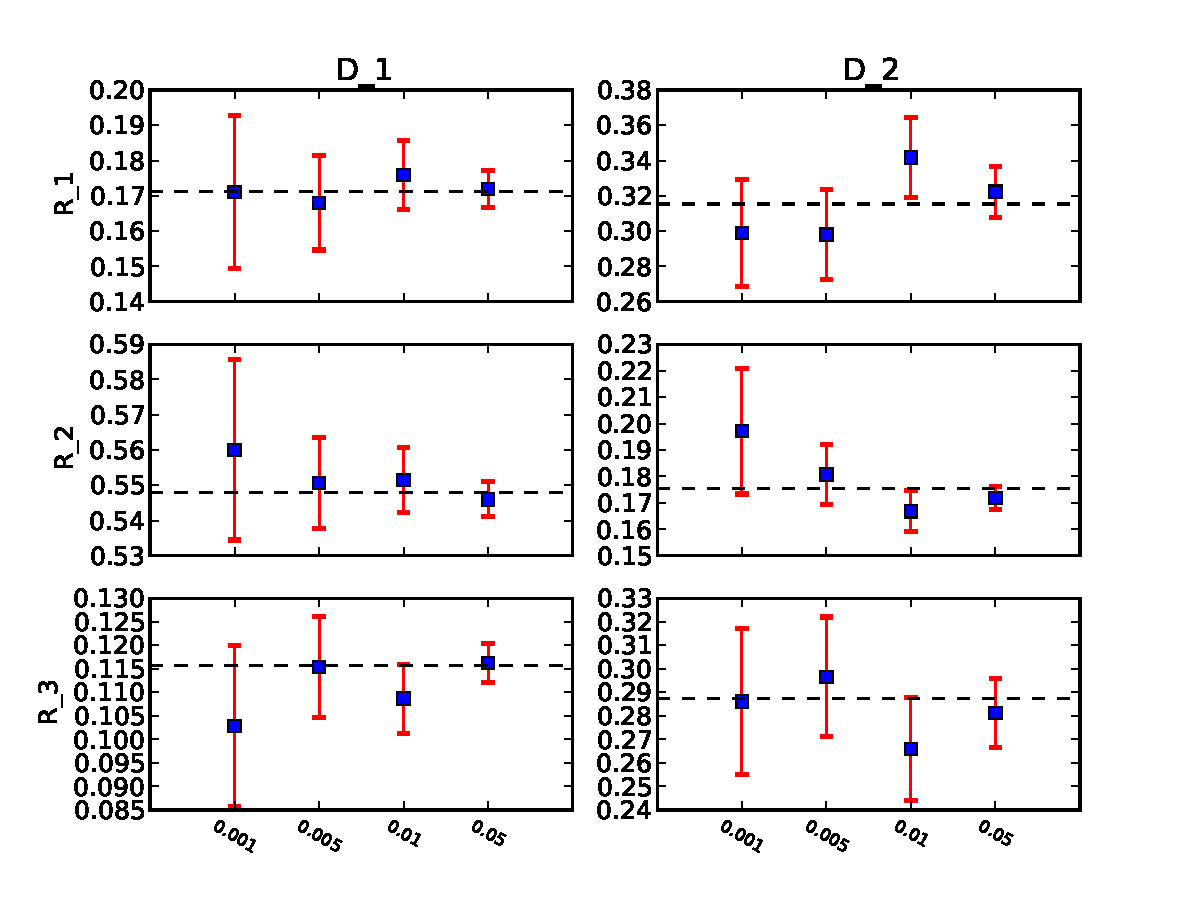
\includegraphics[scale=0.7]{../figures/errors_n100.pdf}
\end{center}
{\scriptsize {\em Notes:} Each row corresponds to the probability region being {\em Notes:} Each row corresponds to the probability region being estimated and each column corresponds to the dataset used to create the posterior distribution. ({\em Black dashed}) is the true statistic.  The x-axis labels indicate the $\epsilon$ size for each run. }
\end{figure}

\begin{figure}[h!]
\caption{SGLD Error Analysis ($n=1$)}
\label{n1}
\begin{center}
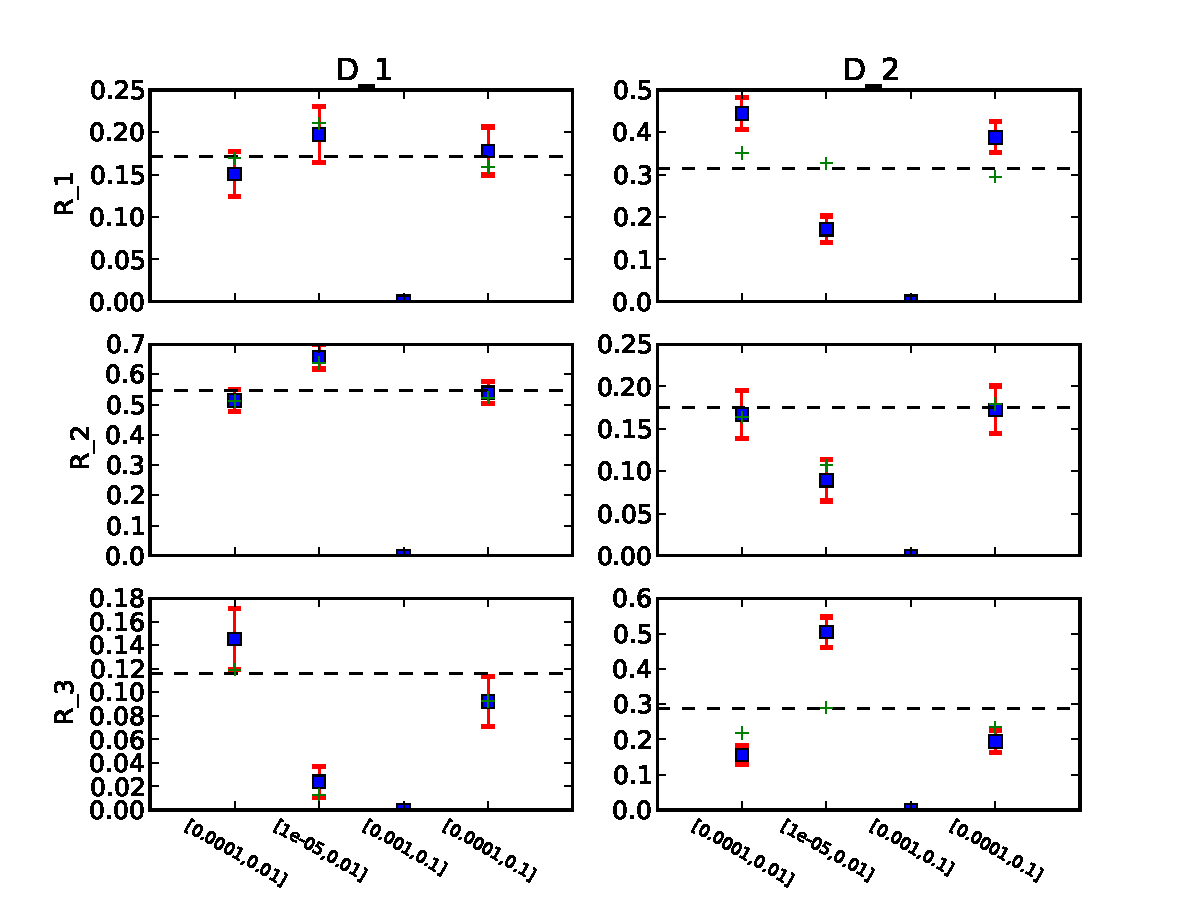
\includegraphics[scale=0.7]{../figures/errors_n1.pdf}
\end{center}
{\scriptsize {\em Notes:} Each row corresponds to the probability region being {\em Notes:} Each row corresponds to the probability region being estimated and each column corresponds to the dataset used to create the posterior distribution. When points are at zero it usually means the sampler did not converge properly and the region was never reached by the sampler.  Each point represents a probability estimate for a region. The red bars indicate the estimated 95\% error bands.  ({\em Black dashed}) is the true statistic.  ({\em Green crosses}) represent the reweighed estimators. Tuples on the x-axis are the minimum and maximum $\epsilon$ values of the annealing schedule. }
\end{figure}
\newpage
\end{section}
\begin{section}{Conclusion}
The SGLD algorithm has some very obvious computational benefits but its performance is variable and very sensitive to annealing schedule and batch size. The hypothesis is that for large and redundant datasets using batches of an appropriate size, the stochastic gradient will be a good approximate of the true gradient.  We see though in our error analysis that the discretization error for SGLD will lead to $O(N/n)$ expected number of rejections which seems to be important enough of an observation to be explored more thoroughly.  This observation suggests that SGLD is inherently biased.  Additionally, the fact that one needs to anneal the step size to zero causes the process to be highly autocorrelated.  The experimental results suggest that the SGLD is in fact not an exact method but it does seem to perform incrementally better for more well behaved distributions.

\cite{AhnBW12} attempts to remedy some of these issues by invoking the so called Bayesian CLT that says when $N$ is big the posterior is approximately normal with covariance equal to the inverse Fisher Information Matrix.  Therefore, one should be able to construct an adaptive MCMC scheme that has this normal distribution as its invariant distribution.  Such a scheme is adaptive in that it incrementally updates the estimate of the Fisher Information matrix. 

What this preliminary paper suggests is that there is presently no free lunch when it comes to sampling complicated and computationally intensive posteriors.  An annealing step size may lead to good posterior maximization but increases autocorrelation time of the chain and causes it to be irreversible.  Avoiding the rejection step which is crucial to guarantee the correctness of most MCMC methods leads to some unintended consequences and even when the probability of rejection goes to zero the number of rejections will be non-trivial and this will lead to biased estimates.  This suggests that an interesting future direction of research might be in developing a theoretically sound approximate rejection step.
\end{section}
\bibliography{biblio}{}
\bibliographystyle{plain}
\newpage
\begin{section}{Appendix}

\begin{figure}[h!]
\caption{SGLD Error Analysis ($n=2$)}
\label{n2}
\begin{center}
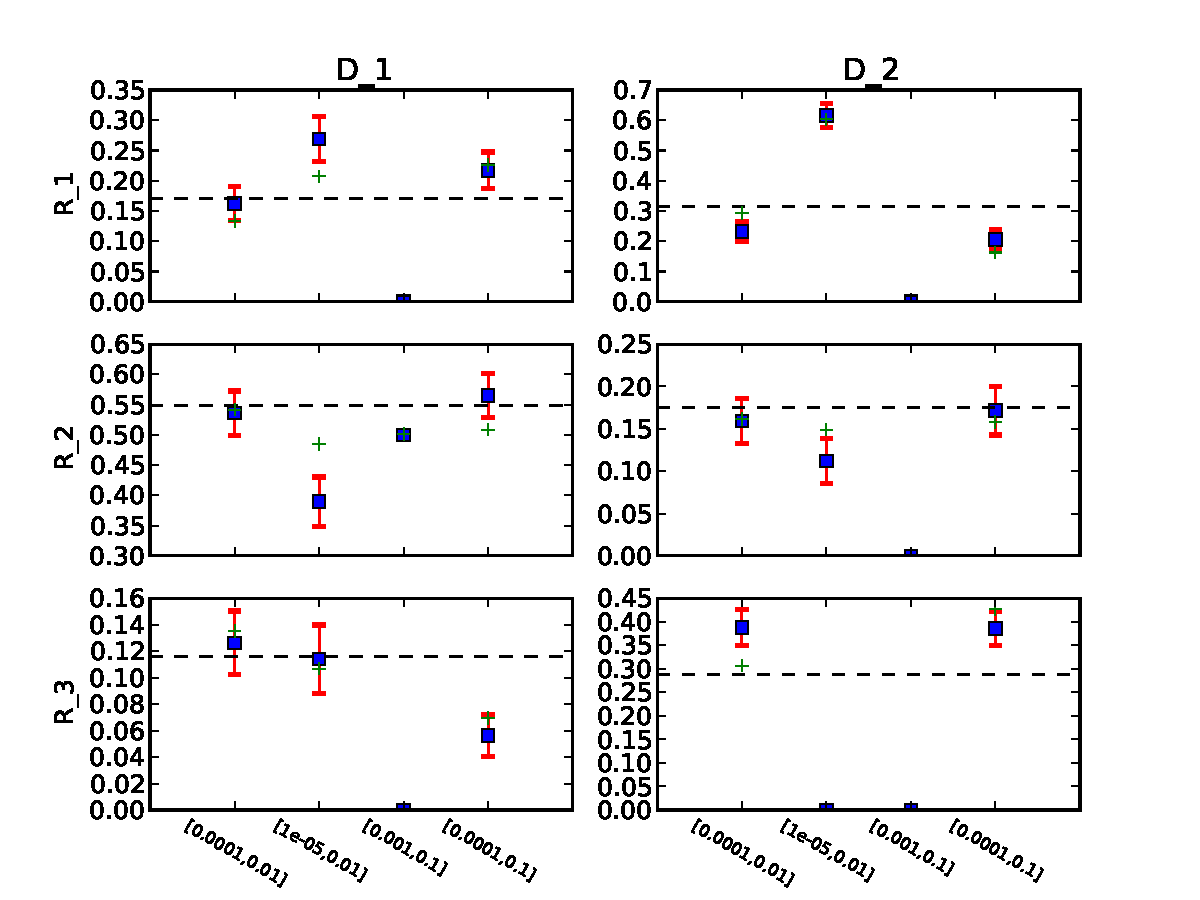
\includegraphics[scale=0.7]{../figures/errors_n2.pdf}
\end{center}
{\scriptsize {\em Notes:} Each row corresponds to the probability region being {\em Notes:} Each row corresponds to the probability region being estimated and each column corresponds to the dataset used to create the posterior distribution. When points are at zero it usually means the sampler did not converge properly and the region was never reached by the sampler.  Each point represents a probability estimate for a region. The red bars indicate the estimated 95\% error bands.  ({\em Black dashed}) is the true statistic.  ({\em Green crosses}) represent the reweighed estimators. Tuples on the x-axis are the minimum and maximum $\epsilon$ values of the annealing schedule. }
\end{figure}

\begin{figure}
\caption{SGLD Error Analysis ($n=4$)}
\label{n4}
\begin{center}
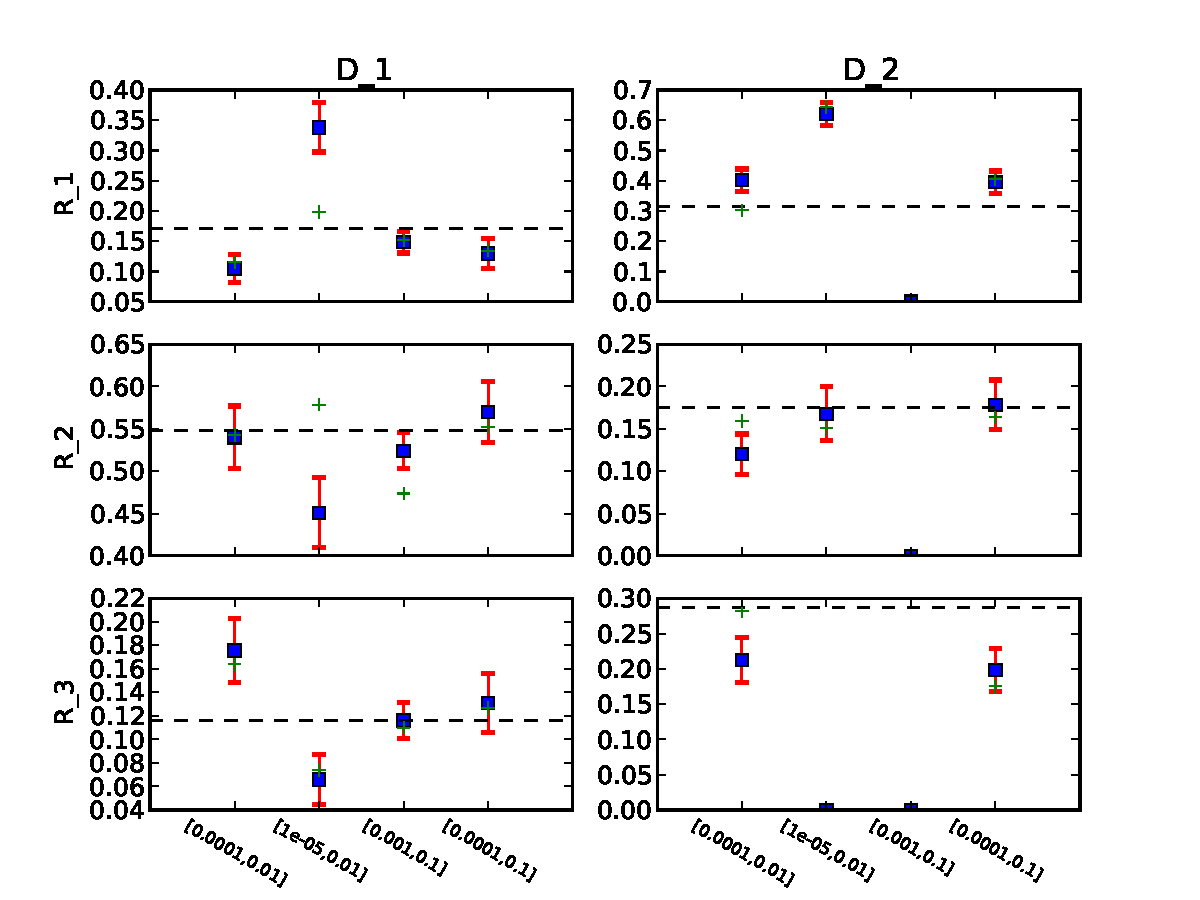
\includegraphics[scale=0.7]{../figures/errors_n4.pdf}
\end{center}
{\scriptsize {\em Notes:} Each row corresponds to the probability region being {\em Notes:} Each row corresponds to the probability region being estimated and each column corresponds to the dataset used to create the posterior distribution. When points are at zero it usually means the sampler did not converge properly and the region was never reached by the sampler.  Each point represents a probability estimate for a region. The red bars indicate the estimated 95\% error bands.  ({\em Black dashed}) is the true statistic.  ({\em Green crosses}) represent the reweighed estimators. Tuples on the x-axis are the minimum and maximum $\epsilon$ values of the annealing schedule. }
\end{figure}

\begin{figure}
\caption{SGLD Error Analysis ($n=8$)}
\label{n8}
\begin{center}
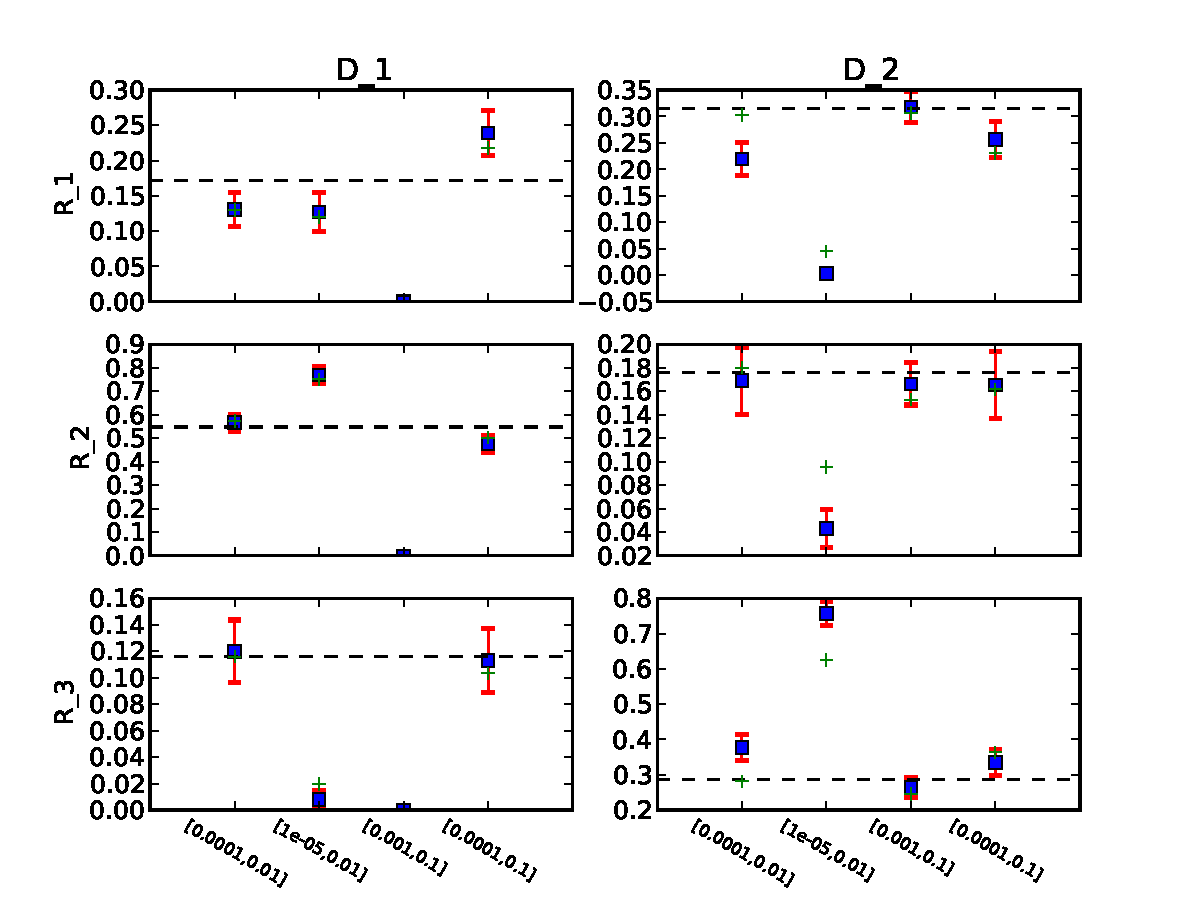
\includegraphics[scale=0.7]{../figures/errors_n8.pdf}
\end{center}
{\scriptsize {\em Notes:} Each row corresponds to the probability region being {\em Notes:} Each row corresponds to the probability region being estimated and each column corresponds to the dataset used to create the posterior distribution. When points are at zero it usually means the sampler did not converge properly and the region was never reached by the sampler.  Each point represents a probability estimate for a region. The red bars indicate the estimated 95\% error bands.  ({\em Black dashed}) is the true statistic.  ({\em Green crosses}) represent the reweighed estimators. Tuples on the x-axis are the minimum and maximum $\epsilon$ values of the annealing schedule. }
\end{figure}

\begin{figure}
\caption{SGLD Error Analysis ($n=16$)}
\label{n16}
\begin{center}
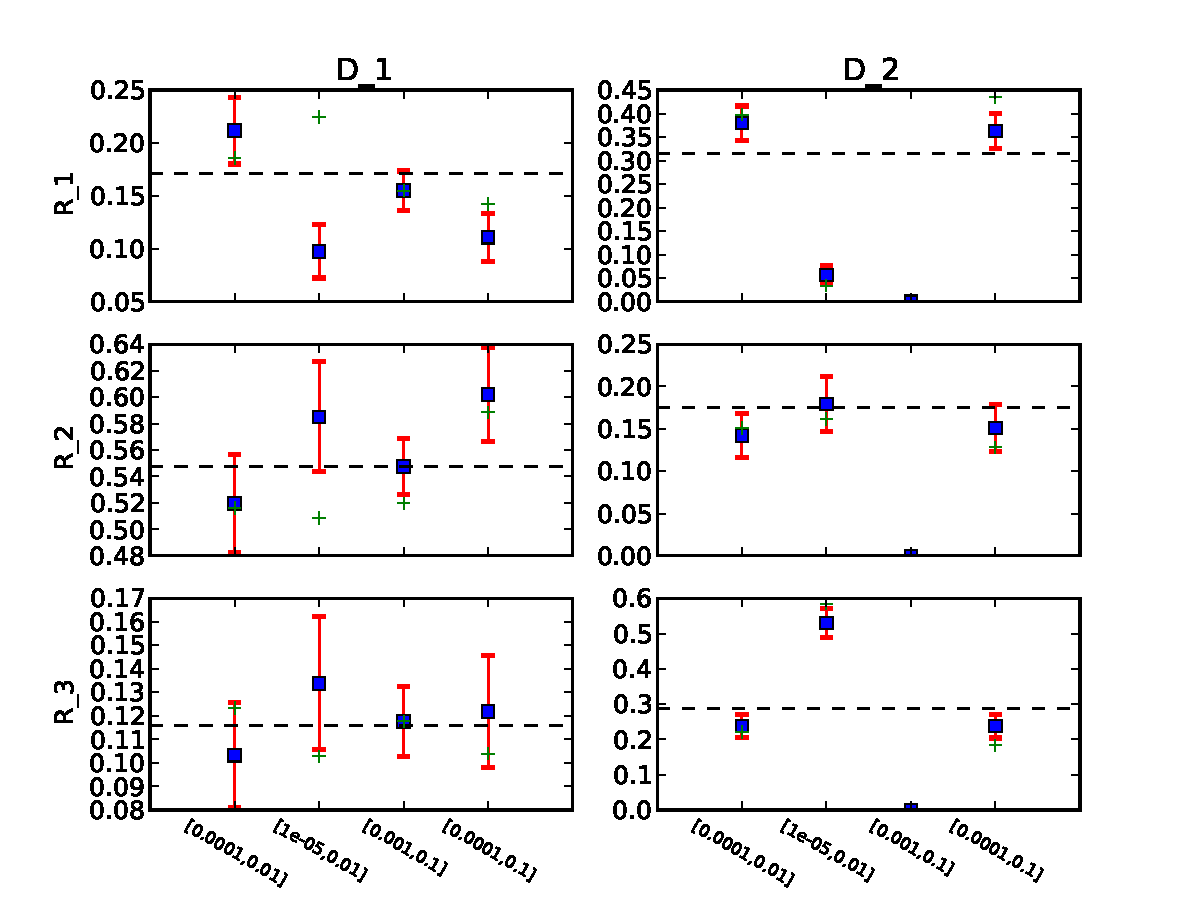
\includegraphics[scale=0.7]{../figures/errors_n16.pdf}
\end{center}
{\scriptsize {\em Notes:} Each row corresponds to the probability region being {\em Notes:} Each row corresponds to the probability region being estimated and each column corresponds to the dataset used to create the posterior distribution. When points are at zero it usually means the sampler did not converge properly and the region was never reached by the sampler.  Each point represents a probability estimate for a region. The red bars indicate the estimated 95\% error bands.  ({\em Black dashed}) is the true statistic.  ({\em Green crosses}) represent the reweighed estimators. Tuples on the x-axis are the minimum and maximum $\epsilon$ values of the annealing schedule. }
\end{figure}
\end{section}

\end{document}